% 图 8.17 克尔效应三种几何：(a) 极向 (b) 纵向 (c) 横向（M 方向不同，光路底图相同）
\documentclass[tikz,border=5pt]{standalone}
\usetikzlibrary{arrows.meta}
\usepackage{amsmath}
\usepackage{bm}
\usepackage{fontspec}
\setmainfont{Times New Roman}
\begin{document}
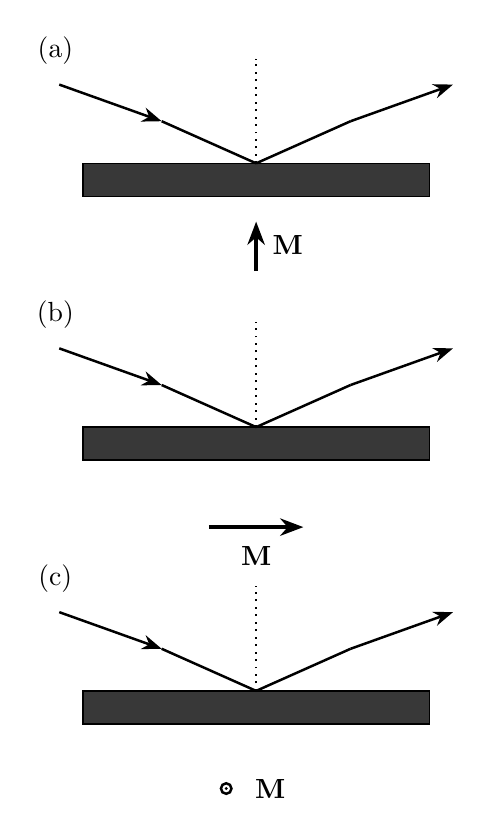
\begin{tikzpicture}[line width=0.8pt,>=Stealth]
% ---------- shared base: film + incident/reflected rays + surface normal ----------
\newcommand{\base}{%
  \fill[black!78] (-2.2,0) rectangle (2.2,0.42);
  \draw[line width=0.5,black] (-2.2,0) rectangle (2.2,0.42);
  \draw[dotted,line width=0.7] (0,0.42) -- (0,1.75);
  \draw[->,line width=0.9] (-2.5,1.42) -- (-1.2,0.955);
  \draw[line width=0.9] (-1.2,0.955) -- (0,0.42);
  \draw[line width=0.9] (0,0.42) -- (1.2,0.955);
  \draw[->,line width=0.9] (1.2,0.955) -- (2.5,1.42);
}
% ---------- (a) polar: M perpendicular to the film plane ----------
\begin{scope}[shift={(0,0)}]
  \base
  \draw[->,line width=1.2] (0,-0.95) -- (0,-0.32);
  \node at (0.4,-0.62) {$\mathbf{M}$};
  \node at (-2.55,1.85) {(a)};
\end{scope}
% ---------- (b) longitudinal: M in the plane of incidence ----------
\begin{scope}[shift={(0,-3.35)}]
  \base
  \draw[->,line width=1.2] (-0.6,-0.85) -- (0.6,-0.85);
  \node at (0,-1.22) {$\mathbf{M}$};
  \node at (-2.55,1.85) {(b)};
\end{scope}
% ---------- (c) transverse: M perpendicular to the plane of incidence ----------
\begin{scope}[shift={(0,-6.7)}]
  \base
  \draw[line width=0.9] (-0.38,-0.82) circle (1.9pt);
  \fill (-0.38,-0.82) circle (0.6pt);
  \node at (0.18,-0.82) {$\mathbf{M}$};
  \node at (-2.55,1.85) {(c)};
\end{scope}
\end{tikzpicture}
\end{document}
